% NeurIPS 2026 main-conference poster: 140 x 90 cm, landscape.
% Compile here: pdflatex poster_camera_ready.tex
% Image-free check: pdflatex -jobname=poster_layout_check '\def\PosterDraft{1}% NeurIPS 2026 main-conference poster: 140 x 90 cm, landscape.
% Compile here: pdflatex poster_camera_ready.tex
% Image-free check: pdflatex -jobname=poster_layout_check '\def\PosterDraft{1}% NeurIPS 2026 main-conference poster: 140 x 90 cm, landscape.
% Compile here: pdflatex poster_camera_ready.tex
% Image-free check: pdflatex -jobname=poster_layout_check '\def\PosterDraft{1}% NeurIPS 2026 main-conference poster: 140 x 90 cm, landscape.
% Compile here: pdflatex poster_camera_ready.tex
% Image-free check: pdflatex -jobname=poster_layout_check '\def\PosterDraft{1}\input{poster_camera_ready.tex}'
\documentclass{article}
\usepackage[paperwidth=140cm,paperheight=90cm,margin=0cm]{geometry}
\usepackage[T1]{fontenc}
\usepackage{lmodern,graphicx,amsmath,amssymb,booktabs}
\usepackage[table]{xcolor}
\usepackage[absolute,overlay]{textpos}
\usepackage{tcolorbox,hyperref,tikz}
\hypersetup{pdftitle={RaPD: Resolution-Agnostic Pixel Diffusion via Semantics-Enriched Implicit Representations},pdfauthor={Yanhao Ge, Shanyan Guan, Weihao Wang, Ying Tai, Mingyu You},hidelinks}
\renewcommand{\familydefault}{\sfdefault}
\pagestyle{empty}
\setlength{\parindent}{0pt}
\setlength{\parskip}{0.3cm}
\definecolor{navy}{HTML}{163654}
\definecolor{accent}{HTML}{D45D32}
\definecolor{soft}{HTML}{F1F5F8}
\definecolor{muted}{HTML}{526474}
\definecolor{line}{HTML}{D6E1E9}
\newcommand{\bodyfont}{\fontsize{25}{32}\selectfont}
\newcommand{\smallfont}{\fontsize{20}{26}\selectfont}
\newcommand{\captiontext}[1]{{\smallfont\color{muted}#1\par}}
\newcommand{\highlight}[1]{{\color{accent}\bfseries #1}}
% width, x, y, height, title, body; dimensions in cm.
\newcommand{\module}[6]{%
\begin{textblock*}{#1cm}(#2cm,#3cm)
\begin{tcolorbox}[width=#1cm,height=#4cm,colback=white,colframe=line,
colbacktitle=navy,coltitle=white,boxrule=1.2pt,arc=0.25cm,
left=0.8cm,right=0.8cm,top=0.65cm,bottom=0.65cm,
fonttitle=\fontsize{32}{38}\selectfont\bfseries,title={#5}]
\bodyfont #6
\end{tcolorbox}\end{textblock*}}
% Draft branch deliberately never calls includegraphics or reads image files.
\newcommand{\posterfigure}[2]{%
\par\noindent\begin{minipage}[c][#2cm][c]{\linewidth}\centering
\ifdefined\PosterDraft
\fcolorbox{line}{soft}{\parbox[c][\dimexpr#2cm-8pt\relax][c]{0.94\linewidth}{\centering\smallfont Image placeholder\\\texttt{\detokenize{#1}}}}
\else
\includegraphics[width=\linewidth,height=#2cm,keepaspectratio]{../figures/#1}
\fi
\end{minipage}\par}
\newcommand{\placeholder}[3]{%
\begin{tcolorbox}[width=#1cm,height=#2cm,colback=soft,colframe=line,
boxrule=1pt,arc=0.2cm,valign=center,halign=center]
\fontsize{22}{27}\selectfont\color{muted}#3\end{tcolorbox}}
\begin{document}
\null
% HEADER: institutional logos | title, authors, affiliations | conference + QR.
\begin{textblock*}{16cm}(2cm,2cm)
\placeholder{16}{3.6}{Tongji University\\LOGO}
\vspace{0.25cm}\placeholder{16}{3.6}{Nanjing University\\LOGO}
\vspace{0.25cm}\placeholder{16}{3.6}{vivo\\LOGO}
\end{textblock*}
\begin{textblock*}{100cm}(20cm,2cm)
\centering
{\fontsize{72}{84}\selectfont\bfseries\color{navy}RaPD: Resolution-Agnostic Pixel Diffusion via\\Semantics-Enriched Implicit Representations\par}
\vspace{0.7cm}
{\fontsize{31}{40}\selectfont Yanhao Ge$^1$\quad Shanyan Guan$^2$\quad Weihao Wang$^{1,2}$\quad Ying Tai$^3$\quad Mingyu You$^{1,4}$\par}
\vspace{0.4cm}
{\fontsize{23}{31}\selectfont
$^1$College of Electronic and Information Engineering, Tongji University\qquad $^2$vivo Mobile Communication Co., Ltd.\qquad $^3$Nanjing University\par
$^4$State Key Laboratory of Autonomous Intelligent Unmanned Systems; Frontiers Science Center for Intelligent Autonomous Systems, Ministry of Education\par}
\vspace{0.4cm}
{\fontsize{29}{36}\selectfont\bfseries\color{accent}Generate one representation. Render at different resolutions.\par}
\end{textblock*}
\begin{textblock*}{16cm}(122cm,2cm)
\placeholder{16}{4.2}{NeurIPS 2026\\LOGO}
\vspace{0.5cm}
\begin{minipage}[t]{7.5cm}\placeholder{7.5}{7.5}{PROJECT\\PAGE\\QR}\end{minipage}\hfill
\begin{minipage}[t]{7.5cm}\placeholder{7.5}{7.5}{CODE\\REPOSITORY\\QR}\end{minipage}
\end{textblock*}
\begin{textblock*}{136cm}(2cm,19cm)
{\color{accent}\rule{136cm}{3pt}}
\end{textblock*}
% LEFT COLUMN: slides_camera_ready.tex, pages 2 and 3.
\module{36}{2}{21}{32}{One representation, different resolutions?}{%
The visual world is \highlight{continuous}, but VAE-latent and pixel-token diffusion operate on \textbf{fixed spatial grids}.
\par Higher resolution means more tokens and more diffusion compute.
\par Coordinate-based decoders support flexible output sizes, but reconstruction-trained latents are not necessarily \highlight{ready for generation}.
\begin{center}
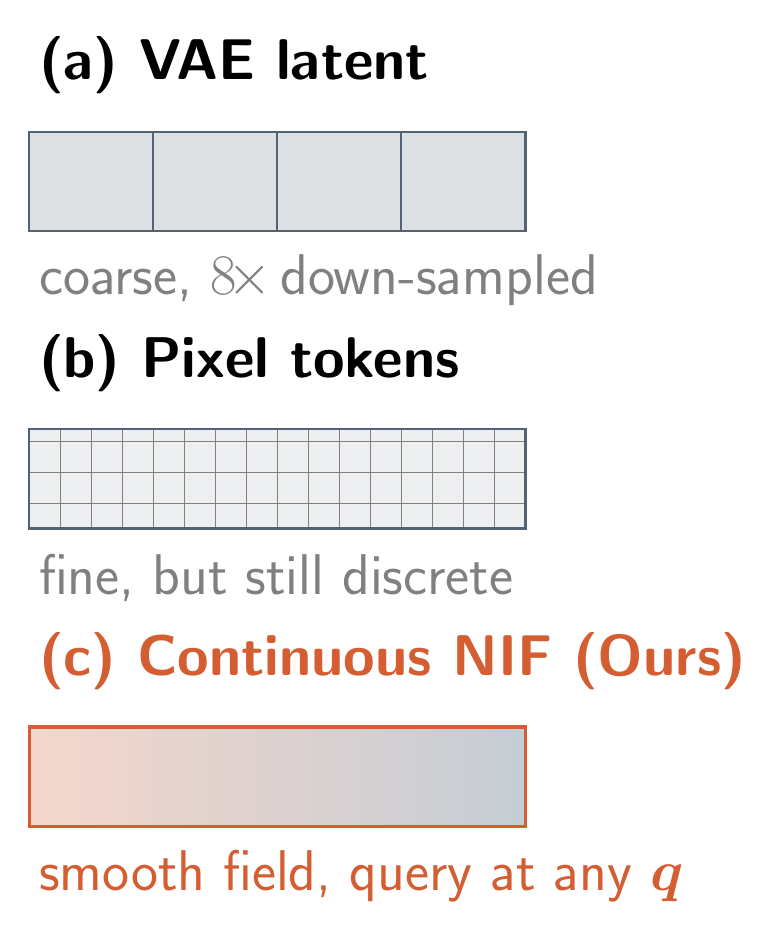
\begin{tikzpicture}[scale=2.1,every node/.style={font=\smallfont}]
        % --- (a) VAE latent: very coarse grid ---
        \node[anchor=west] at (0,3.4) {\textbf{(a) VAE latent}};
        \fill[muted!20] (0,2.4) rectangle (3.0,3.0);
        \draw[step=0.75,muted,thick] (0,2.4) grid (3.0,3.0);
        \draw[muted,thick] (0,2.4) rectangle (3.0,3.0);
        \node[anchor=west,gray] at (0,2.1) {coarse, $8\!\times\!$ down-sampled};
        % --- (b) Pixel tokens: fine grid ---
        \node[anchor=west] at (0,1.6) {\textbf{(b) Pixel tokens}};
        \fill[muted!10] (0,0.6) rectangle (3.0,1.2);
        \draw[step=0.1875,gray,thin] (0,0.6) grid (3.0,1.2);
        \draw[muted,thick] (0,0.6) rectangle (3.0,1.2);
        \node[anchor=west,gray] at (0,0.3) {fine, but still discrete};
        % --- (c) Continuous NIF: smooth gradient, no grid ---
        \node[anchor=west,accent] at (0,-0.2) {\textbf{(c) Continuous NIF (Ours)}};
        \shade[left color=accent!25,right color=navy!25]
          (0,-1.2) rectangle (3.0,-0.6);
        \draw[accent,very thick] (0,-1.2) rectangle (3.0,-0.6);
        \node[accent,anchor=west] at (0,-1.5) {smooth field, query at any $\boldsymbol{q}$};
      \end{tikzpicture}
\end{center}
\textbf{Our question}\par
Can we learn a generation-ready representation that renders at continuous coordinates?}
\module{36}{2}{55}{32}{The reconstruction--generation gap}{%
\posterfigure{exp_render.pdf}{18}
\captiontext{LIIF / CLIF: strong super-resolution reconstruction (top), but weak text-to-image generation (bottom).}
\textbf{Reconstruction training} favors low-level texture rather than semantic structure.
\par Applying diffusion to these latents yields coarse semantics and poor visual fidelity.
\par \textbf{Local decoders} lack inter-pixel reasoning.}
% CENTER COLUMN: method, SRG, CQAR.
\module{46}{40}{21}{26}{Method\quad Learn, generate, then render}{%
\posterfigure{fig1.pdf}{17}
\textbf{Stage-1:} learn semantically guided image-field representations.
\par \textbf{Stage-2:} generate a fixed-size latent with text-conditioned flow matching.
\par \textbf{Inference:} render one latent at different resolutions by changing the query grid.}
\module{46}{40}{49}{16}{SRG\quad Semantic Representation Guidance}{%
\textbf{Semantic distillation.} Pool and project the latent to align with frozen DINOv2 patch features, transferring semantic structure without changing the latent layout.
\par \textbf{Latent-density-aware timestep shift.} Emphasize noisier states during training:
\[
 t=\frac{t_0}{t_0+(1-t_0)s},\qquad s=32.
\]
\highlight{Make reconstruction-oriented latents generation-ready.}}
\module{46}{40}{67}{20}{CQAR\quad Coordinate-Queried Attention Renderer}{%
\posterfigure{fig2.pdf}{12}
Local features, query coordinates and pixel size condition windowed attention over output tokens.
\par \highlight{Inter-pixel reasoning for coherent, arbitrary-resolution rendering.}}
% RIGHT COLUMN: paper Fig. 1 is fig_teaser.pdf (not the method fig1.pdf).
\module{50}{88}{21}{27}{Generation quality and fixed diffusion cost}{%
\begin{minipage}[t]{0.45\linewidth}
\vspace{0pt}
\posterfigure{fig_teaser.pdf}{18}
\captiontext{Paper Fig. 1: GenEval comparison across output resolutions.}
\end{minipage}\hfill
\begin{minipage}[t]{0.52\linewidth}
\vspace{0pt}
{\fontsize{28}{34}\selectfont\bfseries\color{accent}0.86 GenEval / 82.9 DPG\par}
\captiontext{$512^2$; progressive $256\rightarrow512$ training.}
\centering
{\fontsize{20}{27}\selectfont\setlength{\tabcolsep}{9pt}
\begin{tabular}{lcc}\toprule
Method & GenEval & DPG \\\midrule
PixNerd$^\dagger$ & 0.71 & 81.5 \\
PixelGen$^\dagger$ & 0.79 & 80.4 \\
DeCo$^\dagger$ & 0.83 & 81.2 \\
\rowcolor{soft}RaPD ($256\rightarrow512$) & \textbf{0.86} & \textbf{82.9} \\\bottomrule
\end{tabular}\par}
\captiontext{$\dagger$ Same seed and environment.}
\vspace{0.6cm}
\raggedright
{\fontsize{28}{34}\selectfont\bfseries\color{accent}4K in 2.13 seconds\par}
\captiontext{Per image on an NVIDIA B200 GPU.}
\centering
{\fontsize{20}{27}\selectfont\setlength{\tabcolsep}{12pt}
\begin{tabular}{lrr}\toprule
Method & $512^2$ & $4096^2$ \\\midrule
PixelGen & 0.19 s & 61.46 s \\
DeCo & 0.21 s & 62.72 s \\
\rowcolor{soft}RaPD & 0.23 s & \textbf{2.13 s} \\\bottomrule
\end{tabular}\par}
\end{minipage}
\par\vspace{0.3cm}
\textbf{1,024 denoising tokens} at every output size; rendering cost grows with output pixels.
\par\captiontext{High resolution: GenEval 0.85 at both $1024^2$ and $2048^2$ with the $256\rightarrow1024$ model; detailed prompt adherence remains a limitation.}}
\module{50}{88}{50}{23}{Visual results\quad One latent, multiple resolutions}{%
\posterfigure{fig_our_results.pdf}{18}
\captiontext{Training supervision reaches $1024^2$; rendering extends to $2048^2$ and $4096^2$. Only the query grid changes for a fixed generated representation.}}
\module{50}{88}{75}{12}{Why semantic guidance matters}{%
\posterfigure{exp_ablation.pdf}{8}}
\begin{textblock*}{136cm}(2cm,88cm)
\fontsize{18}{23}\selectfont\color{muted}
NeurIPS 2026\quad |\quad Paper 5904\hfill
\href{https://openreview.net/forum?id=BRLhAs1iAm}{openreview.net/forum?id=BRLhAs1iAm}\hfill
Correspondence: myyou@tongji.edu.cn
\end{textblock*}
\end{document}
'
\documentclass{article}
\usepackage[paperwidth=140cm,paperheight=90cm,margin=0cm]{geometry}
\usepackage[T1]{fontenc}
\usepackage{lmodern,graphicx,amsmath,amssymb,booktabs}
\usepackage[table]{xcolor}
\usepackage[absolute,overlay]{textpos}
\usepackage{tcolorbox,hyperref,tikz}
\hypersetup{pdftitle={RaPD: Resolution-Agnostic Pixel Diffusion via Semantics-Enriched Implicit Representations},pdfauthor={Yanhao Ge, Shanyan Guan, Weihao Wang, Ying Tai, Mingyu You},hidelinks}
\renewcommand{\familydefault}{\sfdefault}
\pagestyle{empty}
\setlength{\parindent}{0pt}
\setlength{\parskip}{0.3cm}
\definecolor{navy}{HTML}{163654}
\definecolor{accent}{HTML}{D45D32}
\definecolor{soft}{HTML}{F1F5F8}
\definecolor{muted}{HTML}{526474}
\definecolor{line}{HTML}{D6E1E9}
\newcommand{\bodyfont}{\fontsize{25}{32}\selectfont}
\newcommand{\smallfont}{\fontsize{20}{26}\selectfont}
\newcommand{\captiontext}[1]{{\smallfont\color{muted}#1\par}}
\newcommand{\highlight}[1]{{\color{accent}\bfseries #1}}
% width, x, y, height, title, body; dimensions in cm.
\newcommand{\module}[6]{%
\begin{textblock*}{#1cm}(#2cm,#3cm)
\begin{tcolorbox}[width=#1cm,height=#4cm,colback=white,colframe=line,
colbacktitle=navy,coltitle=white,boxrule=1.2pt,arc=0.25cm,
left=0.8cm,right=0.8cm,top=0.65cm,bottom=0.65cm,
fonttitle=\fontsize{32}{38}\selectfont\bfseries,title={#5}]
\bodyfont #6
\end{tcolorbox}\end{textblock*}}
% Draft branch deliberately never calls includegraphics or reads image files.
\newcommand{\posterfigure}[2]{%
\par\noindent\begin{minipage}[c][#2cm][c]{\linewidth}\centering
\ifdefined\PosterDraft
\fcolorbox{line}{soft}{\parbox[c][\dimexpr#2cm-8pt\relax][c]{0.94\linewidth}{\centering\smallfont Image placeholder\\\texttt{\detokenize{#1}}}}
\else
\includegraphics[width=\linewidth,height=#2cm,keepaspectratio]{../figures/#1}
\fi
\end{minipage}\par}
\newcommand{\placeholder}[3]{%
\begin{tcolorbox}[width=#1cm,height=#2cm,colback=soft,colframe=line,
boxrule=1pt,arc=0.2cm,valign=center,halign=center]
\fontsize{22}{27}\selectfont\color{muted}#3\end{tcolorbox}}
\begin{document}
\null
% HEADER: institutional logos | title, authors, affiliations | conference + QR.
\begin{textblock*}{16cm}(2cm,2cm)
\placeholder{16}{3.6}{Tongji University\\LOGO}
\vspace{0.25cm}\placeholder{16}{3.6}{Nanjing University\\LOGO}
\vspace{0.25cm}\placeholder{16}{3.6}{vivo\\LOGO}
\end{textblock*}
\begin{textblock*}{100cm}(20cm,2cm)
\centering
{\fontsize{72}{84}\selectfont\bfseries\color{navy}RaPD: Resolution-Agnostic Pixel Diffusion via\\Semantics-Enriched Implicit Representations\par}
\vspace{0.7cm}
{\fontsize{31}{40}\selectfont Yanhao Ge$^1$\quad Shanyan Guan$^2$\quad Weihao Wang$^{1,2}$\quad Ying Tai$^3$\quad Mingyu You$^{1,4}$\par}
\vspace{0.4cm}
{\fontsize{23}{31}\selectfont
$^1$College of Electronic and Information Engineering, Tongji University\qquad $^2$vivo Mobile Communication Co., Ltd.\qquad $^3$Nanjing University\par
$^4$State Key Laboratory of Autonomous Intelligent Unmanned Systems; Frontiers Science Center for Intelligent Autonomous Systems, Ministry of Education\par}
\vspace{0.4cm}
{\fontsize{29}{36}\selectfont\bfseries\color{accent}Generate one representation. Render at different resolutions.\par}
\end{textblock*}
\begin{textblock*}{16cm}(122cm,2cm)
\placeholder{16}{4.2}{NeurIPS 2026\\LOGO}
\vspace{0.5cm}
\begin{minipage}[t]{7.5cm}\placeholder{7.5}{7.5}{PROJECT\\PAGE\\QR}\end{minipage}\hfill
\begin{minipage}[t]{7.5cm}\placeholder{7.5}{7.5}{CODE\\REPOSITORY\\QR}\end{minipage}
\end{textblock*}
\begin{textblock*}{136cm}(2cm,19cm)
{\color{accent}\rule{136cm}{3pt}}
\end{textblock*}
% LEFT COLUMN: slides_camera_ready.tex, pages 2 and 3.
\module{36}{2}{21}{32}{One representation, different resolutions?}{%
The visual world is \highlight{continuous}, but VAE-latent and pixel-token diffusion operate on \textbf{fixed spatial grids}.
\par Higher resolution means more tokens and more diffusion compute.
\par Coordinate-based decoders support flexible output sizes, but reconstruction-trained latents are not necessarily \highlight{ready for generation}.
\begin{center}
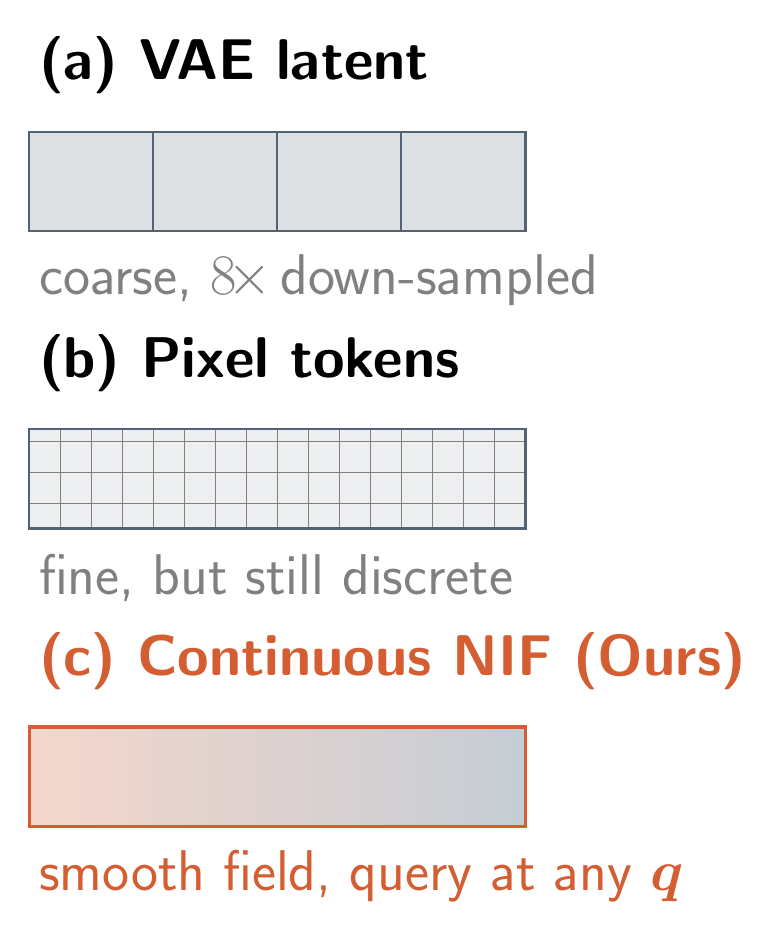
\begin{tikzpicture}[scale=2.1,every node/.style={font=\smallfont}]
        % --- (a) VAE latent: very coarse grid ---
        \node[anchor=west] at (0,3.4) {\textbf{(a) VAE latent}};
        \fill[muted!20] (0,2.4) rectangle (3.0,3.0);
        \draw[step=0.75,muted,thick] (0,2.4) grid (3.0,3.0);
        \draw[muted,thick] (0,2.4) rectangle (3.0,3.0);
        \node[anchor=west,gray] at (0,2.1) {coarse, $8\!\times\!$ down-sampled};
        % --- (b) Pixel tokens: fine grid ---
        \node[anchor=west] at (0,1.6) {\textbf{(b) Pixel tokens}};
        \fill[muted!10] (0,0.6) rectangle (3.0,1.2);
        \draw[step=0.1875,gray,thin] (0,0.6) grid (3.0,1.2);
        \draw[muted,thick] (0,0.6) rectangle (3.0,1.2);
        \node[anchor=west,gray] at (0,0.3) {fine, but still discrete};
        % --- (c) Continuous NIF: smooth gradient, no grid ---
        \node[anchor=west,accent] at (0,-0.2) {\textbf{(c) Continuous NIF (Ours)}};
        \shade[left color=accent!25,right color=navy!25]
          (0,-1.2) rectangle (3.0,-0.6);
        \draw[accent,very thick] (0,-1.2) rectangle (3.0,-0.6);
        \node[accent,anchor=west] at (0,-1.5) {smooth field, query at any $\boldsymbol{q}$};
      \end{tikzpicture}
\end{center}
\textbf{Our question}\par
Can we learn a generation-ready representation that renders at continuous coordinates?}
\module{36}{2}{55}{32}{The reconstruction--generation gap}{%
\posterfigure{exp_render.pdf}{18}
\captiontext{LIIF / CLIF: strong super-resolution reconstruction (top), but weak text-to-image generation (bottom).}
\textbf{Reconstruction training} favors low-level texture rather than semantic structure.
\par Applying diffusion to these latents yields coarse semantics and poor visual fidelity.
\par \textbf{Local decoders} lack inter-pixel reasoning.}
% CENTER COLUMN: method, SRG, CQAR.
\module{46}{40}{21}{26}{Method\quad Learn, generate, then render}{%
\posterfigure{fig1.pdf}{17}
\textbf{Stage-1:} learn semantically guided image-field representations.
\par \textbf{Stage-2:} generate a fixed-size latent with text-conditioned flow matching.
\par \textbf{Inference:} render one latent at different resolutions by changing the query grid.}
\module{46}{40}{49}{16}{SRG\quad Semantic Representation Guidance}{%
\textbf{Semantic distillation.} Pool and project the latent to align with frozen DINOv2 patch features, transferring semantic structure without changing the latent layout.
\par \textbf{Latent-density-aware timestep shift.} Emphasize noisier states during training:
\[
 t=\frac{t_0}{t_0+(1-t_0)s},\qquad s=32.
\]
\highlight{Make reconstruction-oriented latents generation-ready.}}
\module{46}{40}{67}{20}{CQAR\quad Coordinate-Queried Attention Renderer}{%
\posterfigure{fig2.pdf}{12}
Local features, query coordinates and pixel size condition windowed attention over output tokens.
\par \highlight{Inter-pixel reasoning for coherent, arbitrary-resolution rendering.}}
% RIGHT COLUMN: paper Fig. 1 is fig_teaser.pdf (not the method fig1.pdf).
\module{50}{88}{21}{27}{Generation quality and fixed diffusion cost}{%
\begin{minipage}[t]{0.45\linewidth}
\vspace{0pt}
\posterfigure{fig_teaser.pdf}{18}
\captiontext{Paper Fig. 1: GenEval comparison across output resolutions.}
\end{minipage}\hfill
\begin{minipage}[t]{0.52\linewidth}
\vspace{0pt}
{\fontsize{28}{34}\selectfont\bfseries\color{accent}0.86 GenEval / 82.9 DPG\par}
\captiontext{$512^2$; progressive $256\rightarrow512$ training.}
\centering
{\fontsize{20}{27}\selectfont\setlength{\tabcolsep}{9pt}
\begin{tabular}{lcc}\toprule
Method & GenEval & DPG \\\midrule
PixNerd$^\dagger$ & 0.71 & 81.5 \\
PixelGen$^\dagger$ & 0.79 & 80.4 \\
DeCo$^\dagger$ & 0.83 & 81.2 \\
\rowcolor{soft}RaPD ($256\rightarrow512$) & \textbf{0.86} & \textbf{82.9} \\\bottomrule
\end{tabular}\par}
\captiontext{$\dagger$ Same seed and environment.}
\vspace{0.6cm}
\raggedright
{\fontsize{28}{34}\selectfont\bfseries\color{accent}4K in 2.13 seconds\par}
\captiontext{Per image on an NVIDIA B200 GPU.}
\centering
{\fontsize{20}{27}\selectfont\setlength{\tabcolsep}{12pt}
\begin{tabular}{lrr}\toprule
Method & $512^2$ & $4096^2$ \\\midrule
PixelGen & 0.19 s & 61.46 s \\
DeCo & 0.21 s & 62.72 s \\
\rowcolor{soft}RaPD & 0.23 s & \textbf{2.13 s} \\\bottomrule
\end{tabular}\par}
\end{minipage}
\par\vspace{0.3cm}
\textbf{1,024 denoising tokens} at every output size; rendering cost grows with output pixels.
\par\captiontext{High resolution: GenEval 0.85 at both $1024^2$ and $2048^2$ with the $256\rightarrow1024$ model; detailed prompt adherence remains a limitation.}}
\module{50}{88}{50}{23}{Visual results\quad One latent, multiple resolutions}{%
\posterfigure{fig_our_results.pdf}{18}
\captiontext{Training supervision reaches $1024^2$; rendering extends to $2048^2$ and $4096^2$. Only the query grid changes for a fixed generated representation.}}
\module{50}{88}{75}{12}{Why semantic guidance matters}{%
\posterfigure{exp_ablation.pdf}{8}}
\begin{textblock*}{136cm}(2cm,88cm)
\fontsize{18}{23}\selectfont\color{muted}
NeurIPS 2026\quad |\quad Paper 5904\hfill
\href{https://openreview.net/forum?id=BRLhAs1iAm}{openreview.net/forum?id=BRLhAs1iAm}\hfill
Correspondence: myyou@tongji.edu.cn
\end{textblock*}
\end{document}
'
\documentclass{article}
\usepackage[paperwidth=140cm,paperheight=90cm,margin=0cm]{geometry}
\usepackage[T1]{fontenc}
\usepackage{lmodern,graphicx,amsmath,amssymb,booktabs}
\usepackage[table]{xcolor}
\usepackage[absolute,overlay]{textpos}
\usepackage{tcolorbox,hyperref,tikz}
\hypersetup{pdftitle={RaPD: Resolution-Agnostic Pixel Diffusion via Semantics-Enriched Implicit Representations},pdfauthor={Yanhao Ge, Shanyan Guan, Weihao Wang, Ying Tai, Mingyu You},hidelinks}
\renewcommand{\familydefault}{\sfdefault}
\pagestyle{empty}
\setlength{\parindent}{0pt}
\setlength{\parskip}{0.3cm}
\definecolor{navy}{HTML}{163654}
\definecolor{accent}{HTML}{D45D32}
\definecolor{soft}{HTML}{F1F5F8}
\definecolor{muted}{HTML}{526474}
\definecolor{line}{HTML}{D6E1E9}
\newcommand{\bodyfont}{\fontsize{25}{32}\selectfont}
\newcommand{\smallfont}{\fontsize{20}{26}\selectfont}
\newcommand{\captiontext}[1]{{\smallfont\color{muted}#1\par}}
\newcommand{\highlight}[1]{{\color{accent}\bfseries #1}}
% width, x, y, height, title, body; dimensions in cm.
\newcommand{\module}[6]{%
\begin{textblock*}{#1cm}(#2cm,#3cm)
\begin{tcolorbox}[width=#1cm,height=#4cm,colback=white,colframe=line,
colbacktitle=navy,coltitle=white,boxrule=1.2pt,arc=0.25cm,
left=0.8cm,right=0.8cm,top=0.65cm,bottom=0.65cm,
fonttitle=\fontsize{32}{38}\selectfont\bfseries,title={#5}]
\bodyfont #6
\end{tcolorbox}\end{textblock*}}
% Draft branch deliberately never calls includegraphics or reads image files.
\newcommand{\posterfigure}[2]{%
\par\noindent\begin{minipage}[c][#2cm][c]{\linewidth}\centering
\ifdefined\PosterDraft
\fcolorbox{line}{soft}{\parbox[c][\dimexpr#2cm-8pt\relax][c]{0.94\linewidth}{\centering\smallfont Image placeholder\\\texttt{\detokenize{#1}}}}
\else
\includegraphics[width=\linewidth,height=#2cm,keepaspectratio]{../figures/#1}
\fi
\end{minipage}\par}
\newcommand{\placeholder}[3]{%
\begin{tcolorbox}[width=#1cm,height=#2cm,colback=soft,colframe=line,
boxrule=1pt,arc=0.2cm,valign=center,halign=center]
\fontsize{22}{27}\selectfont\color{muted}#3\end{tcolorbox}}
\begin{document}
\null
% HEADER: institutional logos | title, authors, affiliations | conference + QR.
\begin{textblock*}{16cm}(2cm,2cm)
\placeholder{16}{3.6}{Tongji University\\LOGO}
\vspace{0.25cm}\placeholder{16}{3.6}{Nanjing University\\LOGO}
\vspace{0.25cm}\placeholder{16}{3.6}{vivo\\LOGO}
\end{textblock*}
\begin{textblock*}{100cm}(20cm,2cm)
\centering
{\fontsize{72}{84}\selectfont\bfseries\color{navy}RaPD: Resolution-Agnostic Pixel Diffusion via\\Semantics-Enriched Implicit Representations\par}
\vspace{0.7cm}
{\fontsize{31}{40}\selectfont Yanhao Ge$^1$\quad Shanyan Guan$^2$\quad Weihao Wang$^{1,2}$\quad Ying Tai$^3$\quad Mingyu You$^{1,4}$\par}
\vspace{0.4cm}
{\fontsize{23}{31}\selectfont
$^1$College of Electronic and Information Engineering, Tongji University\qquad $^2$vivo Mobile Communication Co., Ltd.\qquad $^3$Nanjing University\par
$^4$State Key Laboratory of Autonomous Intelligent Unmanned Systems; Frontiers Science Center for Intelligent Autonomous Systems, Ministry of Education\par}
\vspace{0.4cm}
{\fontsize{29}{36}\selectfont\bfseries\color{accent}Generate one representation. Render at different resolutions.\par}
\end{textblock*}
\begin{textblock*}{16cm}(122cm,2cm)
\placeholder{16}{4.2}{NeurIPS 2026\\LOGO}
\vspace{0.5cm}
\begin{minipage}[t]{7.5cm}\placeholder{7.5}{7.5}{PROJECT\\PAGE\\QR}\end{minipage}\hfill
\begin{minipage}[t]{7.5cm}\placeholder{7.5}{7.5}{CODE\\REPOSITORY\\QR}\end{minipage}
\end{textblock*}
\begin{textblock*}{136cm}(2cm,19cm)
{\color{accent}\rule{136cm}{3pt}}
\end{textblock*}
% LEFT COLUMN: slides_camera_ready.tex, pages 2 and 3.
\module{36}{2}{21}{32}{One representation, different resolutions?}{%
The visual world is \highlight{continuous}, but VAE-latent and pixel-token diffusion operate on \textbf{fixed spatial grids}.
\par Higher resolution means more tokens and more diffusion compute.
\par Coordinate-based decoders support flexible output sizes, but reconstruction-trained latents are not necessarily \highlight{ready for generation}.
\begin{center}
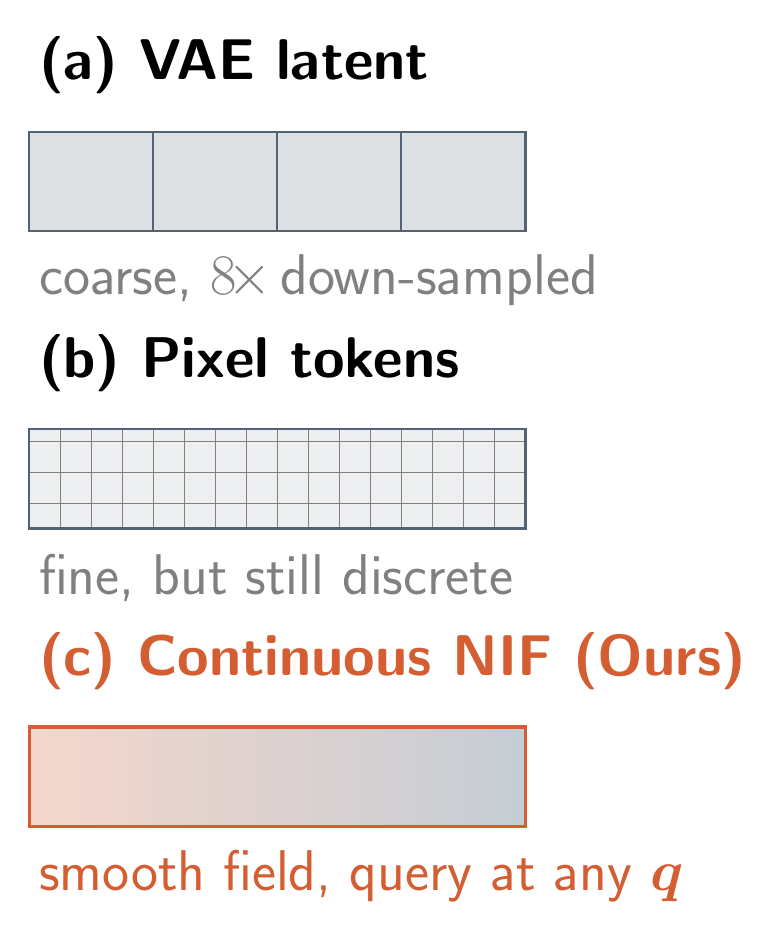
\begin{tikzpicture}[scale=2.1,every node/.style={font=\smallfont}]
        % --- (a) VAE latent: very coarse grid ---
        \node[anchor=west] at (0,3.4) {\textbf{(a) VAE latent}};
        \fill[muted!20] (0,2.4) rectangle (3.0,3.0);
        \draw[step=0.75,muted,thick] (0,2.4) grid (3.0,3.0);
        \draw[muted,thick] (0,2.4) rectangle (3.0,3.0);
        \node[anchor=west,gray] at (0,2.1) {coarse, $8\!\times\!$ down-sampled};
        % --- (b) Pixel tokens: fine grid ---
        \node[anchor=west] at (0,1.6) {\textbf{(b) Pixel tokens}};
        \fill[muted!10] (0,0.6) rectangle (3.0,1.2);
        \draw[step=0.1875,gray,thin] (0,0.6) grid (3.0,1.2);
        \draw[muted,thick] (0,0.6) rectangle (3.0,1.2);
        \node[anchor=west,gray] at (0,0.3) {fine, but still discrete};
        % --- (c) Continuous NIF: smooth gradient, no grid ---
        \node[anchor=west,accent] at (0,-0.2) {\textbf{(c) Continuous NIF (Ours)}};
        \shade[left color=accent!25,right color=navy!25]
          (0,-1.2) rectangle (3.0,-0.6);
        \draw[accent,very thick] (0,-1.2) rectangle (3.0,-0.6);
        \node[accent,anchor=west] at (0,-1.5) {smooth field, query at any $\boldsymbol{q}$};
      \end{tikzpicture}
\end{center}
\textbf{Our question}\par
Can we learn a generation-ready representation that renders at continuous coordinates?}
\module{36}{2}{55}{32}{The reconstruction--generation gap}{%
\posterfigure{exp_render.pdf}{18}
\captiontext{LIIF / CLIF: strong super-resolution reconstruction (top), but weak text-to-image generation (bottom).}
\textbf{Reconstruction training} favors low-level texture rather than semantic structure.
\par Applying diffusion to these latents yields coarse semantics and poor visual fidelity.
\par \textbf{Local decoders} lack inter-pixel reasoning.}
% CENTER COLUMN: method, SRG, CQAR.
\module{46}{40}{21}{26}{Method\quad Learn, generate, then render}{%
\posterfigure{fig1.pdf}{17}
\textbf{Stage-1:} learn semantically guided image-field representations.
\par \textbf{Stage-2:} generate a fixed-size latent with text-conditioned flow matching.
\par \textbf{Inference:} render one latent at different resolutions by changing the query grid.}
\module{46}{40}{49}{16}{SRG\quad Semantic Representation Guidance}{%
\textbf{Semantic distillation.} Pool and project the latent to align with frozen DINOv2 patch features, transferring semantic structure without changing the latent layout.
\par \textbf{Latent-density-aware timestep shift.} Emphasize noisier states during training:
\[
 t=\frac{t_0}{t_0+(1-t_0)s},\qquad s=32.
\]
\highlight{Make reconstruction-oriented latents generation-ready.}}
\module{46}{40}{67}{20}{CQAR\quad Coordinate-Queried Attention Renderer}{%
\posterfigure{fig2.pdf}{12}
Local features, query coordinates and pixel size condition windowed attention over output tokens.
\par \highlight{Inter-pixel reasoning for coherent, arbitrary-resolution rendering.}}
% RIGHT COLUMN: paper Fig. 1 is fig_teaser.pdf (not the method fig1.pdf).
\module{50}{88}{21}{27}{Generation quality and fixed diffusion cost}{%
\begin{minipage}[t]{0.45\linewidth}
\vspace{0pt}
\posterfigure{fig_teaser.pdf}{18}
\captiontext{Paper Fig. 1: GenEval comparison across output resolutions.}
\end{minipage}\hfill
\begin{minipage}[t]{0.52\linewidth}
\vspace{0pt}
{\fontsize{28}{34}\selectfont\bfseries\color{accent}0.86 GenEval / 82.9 DPG\par}
\captiontext{$512^2$; progressive $256\rightarrow512$ training.}
\centering
{\fontsize{20}{27}\selectfont\setlength{\tabcolsep}{9pt}
\begin{tabular}{lcc}\toprule
Method & GenEval & DPG \\\midrule
PixNerd$^\dagger$ & 0.71 & 81.5 \\
PixelGen$^\dagger$ & 0.79 & 80.4 \\
DeCo$^\dagger$ & 0.83 & 81.2 \\
\rowcolor{soft}RaPD ($256\rightarrow512$) & \textbf{0.86} & \textbf{82.9} \\\bottomrule
\end{tabular}\par}
\captiontext{$\dagger$ Same seed and environment.}
\vspace{0.6cm}
\raggedright
{\fontsize{28}{34}\selectfont\bfseries\color{accent}4K in 2.13 seconds\par}
\captiontext{Per image on an NVIDIA B200 GPU.}
\centering
{\fontsize{20}{27}\selectfont\setlength{\tabcolsep}{12pt}
\begin{tabular}{lrr}\toprule
Method & $512^2$ & $4096^2$ \\\midrule
PixelGen & 0.19 s & 61.46 s \\
DeCo & 0.21 s & 62.72 s \\
\rowcolor{soft}RaPD & 0.23 s & \textbf{2.13 s} \\\bottomrule
\end{tabular}\par}
\end{minipage}
\par\vspace{0.3cm}
\textbf{1,024 denoising tokens} at every output size; rendering cost grows with output pixels.
\par\captiontext{High resolution: GenEval 0.85 at both $1024^2$ and $2048^2$ with the $256\rightarrow1024$ model; detailed prompt adherence remains a limitation.}}
\module{50}{88}{50}{23}{Visual results\quad One latent, multiple resolutions}{%
\posterfigure{fig_our_results.pdf}{18}
\captiontext{Training supervision reaches $1024^2$; rendering extends to $2048^2$ and $4096^2$. Only the query grid changes for a fixed generated representation.}}
\module{50}{88}{75}{12}{Why semantic guidance matters}{%
\posterfigure{exp_ablation.pdf}{8}}
\begin{textblock*}{136cm}(2cm,88cm)
\fontsize{18}{23}\selectfont\color{muted}
NeurIPS 2026\quad |\quad Paper 5904\hfill
\href{https://openreview.net/forum?id=BRLhAs1iAm}{openreview.net/forum?id=BRLhAs1iAm}\hfill
Correspondence: myyou@tongji.edu.cn
\end{textblock*}
\end{document}
'
\documentclass{article}
\usepackage[paperwidth=140cm,paperheight=90cm,margin=0cm]{geometry}
\usepackage[T1]{fontenc}
\usepackage{lmodern,graphicx,amsmath,amssymb,booktabs}
\usepackage[table]{xcolor}
\usepackage[absolute,overlay]{textpos}
\usepackage{tcolorbox,hyperref,tikz}
\hypersetup{pdftitle={RaPD: Resolution-Agnostic Pixel Diffusion via Semantics-Enriched Implicit Representations},pdfauthor={Yanhao Ge, Shanyan Guan, Weihao Wang, Ying Tai, Mingyu You},hidelinks}
\renewcommand{\familydefault}{\sfdefault}
\pagestyle{empty}
\setlength{\parindent}{0pt}
\setlength{\parskip}{0.3cm}
\definecolor{navy}{HTML}{163654}
\definecolor{accent}{HTML}{D45D32}
\definecolor{soft}{HTML}{F1F5F8}
\definecolor{muted}{HTML}{526474}
\definecolor{line}{HTML}{D6E1E9}
\newcommand{\bodyfont}{\fontsize{25}{32}\selectfont}
\newcommand{\smallfont}{\fontsize{20}{26}\selectfont}
\newcommand{\captiontext}[1]{{\smallfont\color{muted}#1\par}}
\newcommand{\highlight}[1]{{\color{accent}\bfseries #1}}
% width, x, y, height, title, body; dimensions in cm.
\newcommand{\module}[6]{%
\begin{textblock*}{#1cm}(#2cm,#3cm)
\begin{tcolorbox}[width=#1cm,height=#4cm,colback=white,colframe=line,
colbacktitle=navy,coltitle=white,boxrule=1.2pt,arc=0.25cm,
left=0.8cm,right=0.8cm,top=0.65cm,bottom=0.65cm,
fonttitle=\fontsize{32}{38}\selectfont\bfseries,title={#5}]
\bodyfont #6
\end{tcolorbox}\end{textblock*}}
% Draft branch deliberately never calls includegraphics or reads image files.
\newcommand{\posterfigure}[2]{%
\par\noindent\begin{minipage}[c][#2cm][c]{\linewidth}\centering
\ifdefined\PosterDraft
\fcolorbox{line}{soft}{\parbox[c][\dimexpr#2cm-8pt\relax][c]{0.94\linewidth}{\centering\smallfont Image placeholder\\\texttt{\detokenize{#1}}}}
\else
\includegraphics[width=\linewidth,height=#2cm,keepaspectratio]{../figures/#1}
\fi
\end{minipage}\par}
\newcommand{\placeholder}[3]{%
\begin{tcolorbox}[width=#1cm,height=#2cm,colback=soft,colframe=line,
boxrule=1pt,arc=0.2cm,valign=center,halign=center]
\fontsize{22}{27}\selectfont\color{muted}#3\end{tcolorbox}}
\begin{document}
\null
% HEADER: institutional logos | title, authors, affiliations | conference + QR.
\begin{textblock*}{16cm}(2cm,2cm)
\placeholder{16}{3.6}{Tongji University\\LOGO}
\vspace{0.25cm}\placeholder{16}{3.6}{Nanjing University\\LOGO}
\vspace{0.25cm}\placeholder{16}{3.6}{vivo\\LOGO}
\end{textblock*}
\begin{textblock*}{100cm}(20cm,2cm)
\centering
{\fontsize{72}{84}\selectfont\bfseries\color{navy}RaPD: Resolution-Agnostic Pixel Diffusion via\\Semantics-Enriched Implicit Representations\par}
\vspace{0.7cm}
{\fontsize{31}{40}\selectfont Yanhao Ge$^1$\quad Shanyan Guan$^2$\quad Weihao Wang$^{1,2}$\quad Ying Tai$^3$\quad Mingyu You$^{1,4}$\par}
\vspace{0.4cm}
{\fontsize{23}{31}\selectfont
$^1$College of Electronic and Information Engineering, Tongji University\qquad $^2$vivo Mobile Communication Co., Ltd.\qquad $^3$Nanjing University\par
$^4$State Key Laboratory of Autonomous Intelligent Unmanned Systems; Frontiers Science Center for Intelligent Autonomous Systems, Ministry of Education\par}
\vspace{0.4cm}
{\fontsize{29}{36}\selectfont\bfseries\color{accent}Generate one representation. Render at different resolutions.\par}
\end{textblock*}
\begin{textblock*}{16cm}(122cm,2cm)
\placeholder{16}{4.2}{NeurIPS 2026\\LOGO}
\vspace{0.5cm}
\begin{minipage}[t]{7.5cm}\placeholder{7.5}{7.5}{PROJECT\\PAGE\\QR}\end{minipage}\hfill
\begin{minipage}[t]{7.5cm}\placeholder{7.5}{7.5}{CODE\\REPOSITORY\\QR}\end{minipage}
\end{textblock*}
\begin{textblock*}{136cm}(2cm,19cm)
{\color{accent}\rule{136cm}{3pt}}
\end{textblock*}
% LEFT COLUMN: slides_camera_ready.tex, pages 2 and 3.
\module{36}{2}{21}{32}{One representation, different resolutions?}{%
The visual world is \highlight{continuous}, but VAE-latent and pixel-token diffusion operate on \textbf{fixed spatial grids}.
\par Higher resolution means more tokens and more diffusion compute.
\par Coordinate-based decoders support flexible output sizes, but reconstruction-trained latents are not necessarily \highlight{ready for generation}.
\begin{center}
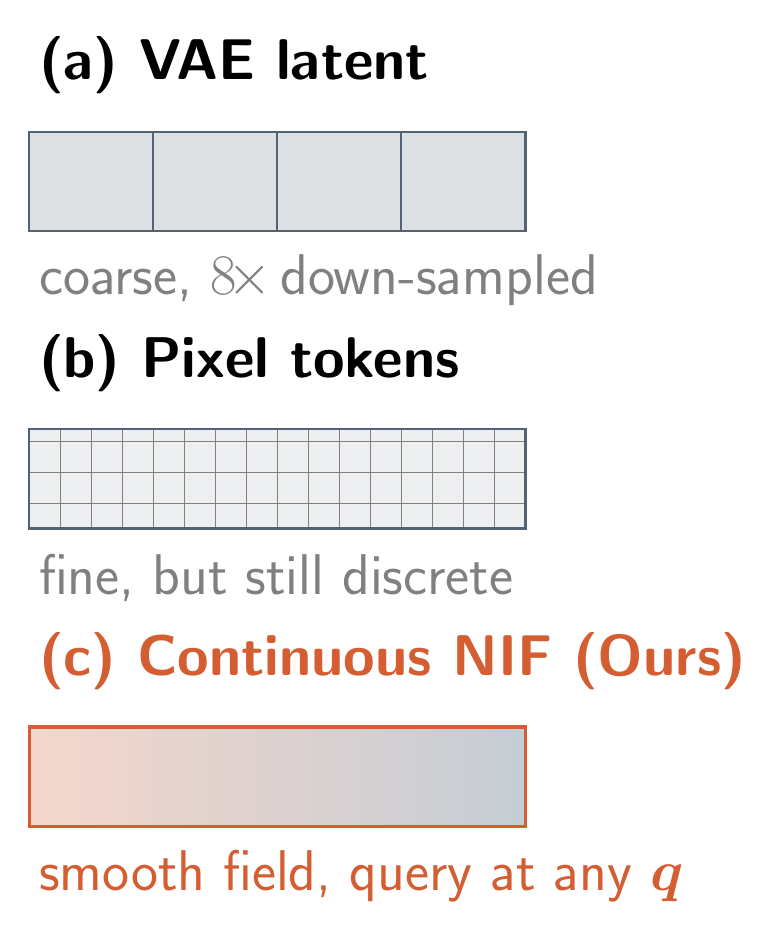
\begin{tikzpicture}[scale=2.1,every node/.style={font=\smallfont}]
        % --- (a) VAE latent: very coarse grid ---
        \node[anchor=west] at (0,3.4) {\textbf{(a) VAE latent}};
        \fill[muted!20] (0,2.4) rectangle (3.0,3.0);
        \draw[step=0.75,muted,thick] (0,2.4) grid (3.0,3.0);
        \draw[muted,thick] (0,2.4) rectangle (3.0,3.0);
        \node[anchor=west,gray] at (0,2.1) {coarse, $8\!\times\!$ down-sampled};
        % --- (b) Pixel tokens: fine grid ---
        \node[anchor=west] at (0,1.6) {\textbf{(b) Pixel tokens}};
        \fill[muted!10] (0,0.6) rectangle (3.0,1.2);
        \draw[step=0.1875,gray,thin] (0,0.6) grid (3.0,1.2);
        \draw[muted,thick] (0,0.6) rectangle (3.0,1.2);
        \node[anchor=west,gray] at (0,0.3) {fine, but still discrete};
        % --- (c) Continuous NIF: smooth gradient, no grid ---
        \node[anchor=west,accent] at (0,-0.2) {\textbf{(c) Continuous NIF (Ours)}};
        \shade[left color=accent!25,right color=navy!25]
          (0,-1.2) rectangle (3.0,-0.6);
        \draw[accent,very thick] (0,-1.2) rectangle (3.0,-0.6);
        \node[accent,anchor=west] at (0,-1.5) {smooth field, query at any $\boldsymbol{q}$};
      \end{tikzpicture}
\end{center}
\textbf{Our question}\par
Can we learn a generation-ready representation that renders at continuous coordinates?}
\module{36}{2}{55}{32}{The reconstruction--generation gap}{%
\posterfigure{exp_render.pdf}{18}
\captiontext{LIIF / CLIF: strong super-resolution reconstruction (top), but weak text-to-image generation (bottom).}
\textbf{Reconstruction training} favors low-level texture rather than semantic structure.
\par Applying diffusion to these latents yields coarse semantics and poor visual fidelity.
\par \textbf{Local decoders} lack inter-pixel reasoning.}
% CENTER COLUMN: method, SRG, CQAR.
\module{46}{40}{21}{26}{Method\quad Learn, generate, then render}{%
\posterfigure{fig1.pdf}{17}
\textbf{Stage-1:} learn semantically guided image-field representations.
\par \textbf{Stage-2:} generate a fixed-size latent with text-conditioned flow matching.
\par \textbf{Inference:} render one latent at different resolutions by changing the query grid.}
\module{46}{40}{49}{16}{SRG\quad Semantic Representation Guidance}{%
\textbf{Semantic distillation.} Pool and project the latent to align with frozen DINOv2 patch features, transferring semantic structure without changing the latent layout.
\par \textbf{Latent-density-aware timestep shift.} Emphasize noisier states during training:
\[
 t=\frac{t_0}{t_0+(1-t_0)s},\qquad s=32.
\]
\highlight{Make reconstruction-oriented latents generation-ready.}}
\module{46}{40}{67}{20}{CQAR\quad Coordinate-Queried Attention Renderer}{%
\posterfigure{fig2.pdf}{12}
Local features, query coordinates and pixel size condition windowed attention over output tokens.
\par \highlight{Inter-pixel reasoning for coherent, arbitrary-resolution rendering.}}
% RIGHT COLUMN: paper Fig. 1 is fig_teaser.pdf (not the method fig1.pdf).
\module{50}{88}{21}{27}{Generation quality and fixed diffusion cost}{%
\begin{minipage}[t]{0.45\linewidth}
\vspace{0pt}
\posterfigure{fig_teaser.pdf}{18}
\captiontext{Paper Fig. 1: GenEval comparison across output resolutions.}
\end{minipage}\hfill
\begin{minipage}[t]{0.52\linewidth}
\vspace{0pt}
{\fontsize{28}{34}\selectfont\bfseries\color{accent}0.86 GenEval / 82.9 DPG\par}
\captiontext{$512^2$; progressive $256\rightarrow512$ training.}
\centering
{\fontsize{20}{27}\selectfont\setlength{\tabcolsep}{9pt}
\begin{tabular}{lcc}\toprule
Method & GenEval & DPG \\\midrule
PixNerd$^\dagger$ & 0.71 & 81.5 \\
PixelGen$^\dagger$ & 0.79 & 80.4 \\
DeCo$^\dagger$ & 0.83 & 81.2 \\
\rowcolor{soft}RaPD ($256\rightarrow512$) & \textbf{0.86} & \textbf{82.9} \\\bottomrule
\end{tabular}\par}
\captiontext{$\dagger$ Same seed and environment.}
\vspace{0.6cm}
\raggedright
{\fontsize{28}{34}\selectfont\bfseries\color{accent}4K in 2.13 seconds\par}
\captiontext{Per image on an NVIDIA B200 GPU.}
\centering
{\fontsize{20}{27}\selectfont\setlength{\tabcolsep}{12pt}
\begin{tabular}{lrr}\toprule
Method & $512^2$ & $4096^2$ \\\midrule
PixelGen & 0.19 s & 61.46 s \\
DeCo & 0.21 s & 62.72 s \\
\rowcolor{soft}RaPD & 0.23 s & \textbf{2.13 s} \\\bottomrule
\end{tabular}\par}
\end{minipage}
\par\vspace{0.3cm}
\textbf{1,024 denoising tokens} at every output size; rendering cost grows with output pixels.
\par\captiontext{High resolution: GenEval 0.85 at both $1024^2$ and $2048^2$ with the $256\rightarrow1024$ model; detailed prompt adherence remains a limitation.}}
\module{50}{88}{50}{23}{Visual results\quad One latent, multiple resolutions}{%
\posterfigure{fig_our_results.pdf}{18}
\captiontext{Training supervision reaches $1024^2$; rendering extends to $2048^2$ and $4096^2$. Only the query grid changes for a fixed generated representation.}}
\module{50}{88}{75}{12}{Why semantic guidance matters}{%
\posterfigure{exp_ablation.pdf}{8}}
\begin{textblock*}{136cm}(2cm,88cm)
\fontsize{18}{23}\selectfont\color{muted}
NeurIPS 2026\quad |\quad Paper 5904\hfill
\href{https://openreview.net/forum?id=BRLhAs1iAm}{openreview.net/forum?id=BRLhAs1iAm}\hfill
Correspondence: myyou@tongji.edu.cn
\end{textblock*}
\end{document}
